% !TeX program = lualatex
% Using VimTeX, you need to reload the plugin (\lx) after having saved the document in order to use LuaLaTeX (thanks to the line above)

\documentclass[a4paper]{book}

% Expanded on !p snip.rv = get_formatted_date() at !p snip.rv = get_formatted_time().

\usepackage{style}

\title{Computer System}
\author{Arthur Herbette}
\date{Tuesday 17 February 2026}

\begin{document}
\maketitle

\newpage
\tableofcontents
\newpage
\section{Memory Virtualisation}
The goal of memory virtualisation is to offer a cpu to deal with more than one user on the same memory. The issue we had without and virtualisation was that. Assume I am user A and I want to steal data from user B. All I need to do is just to scan the whole memory until I find the part that belong to user B process. This is not safe. In order to solve this issue we can introduce virtualisation, the principle is to create a virtual memory for each process. Each process has its own virtual memory, which maps to a physical memory, every process therefore has its own part of the physical memory and each process doesn't know the physical memory behind.\\
$ $\\
A process references memory using \important{virtual} addresses, and \textbf{under the covers}, each virtual memory address is translated to a physical (real) memory address.
\begin{parag}{How}
    Now we can see that the idea is nice however, how do we implement it? Do we allocate a contiguous part of memory for each process? Do we have some part of memory but fixed size, some part of memory that are not of fixed size?\\
	$ $\\
	Let us go one by one and see the pros and cons
\end{parag}

\begin{parag}{Base and Bound}
    In this case, the pros is that it is fairly easy to translate, all we have to do is adding the base to the virtual address. Imagine that the physical memory (the block for the process) starts at \texttt{0x80000}, then when the process makes a load instruction at address \texttt{0x10}, all we have to do it to look in the physical memory at address \texttt{0x80010}.\\
	The issue with that is fragmentation, imagine that we have a contiguous blablabla, for each processes P1, P2, P3, ... The issue we will have is imagine now P2 get killed, there is now a \texttt{0x400} hole in the memory. Now imagine that we want to fork a process that requests \texttt{0x900} as the size of his memory. In this case we cannot put it in there and we have to look outside. We have contiguous physical memory areas that are free but are too small to store a complete memory image. This is a result of requiring that each memory image need to be stored in a contiguous physical memory area. This results in an big inefficiency, a waste of physical memory.
\end{parag}

\begin{parag}{Chunks}
    Now there is a couple way of doing it in chunks we can either:
	\begin{itemize}
	    \item \textbf{Segmentation}: variable sized chunks (segments)
	    \item \textbf{Paging}: same sized chunks (frames)
	\end{itemize}
	The base and bound method we have seen before here is just a crude form of the segmentation, a segmentation with only one chunk.\\
	$ $\\
	So as we can see here those are safe and now we don't have issues as before. Let us take the example of paging, as in this case every frames has a fixed size, this implies that we when freeing memory of a process, this doesn't hurt our physical memory as every frame here can be reused for other processes, we don't have any waste of physical memory. The issue however is that they are of fixed size, this implies that imagine this size is \texttt{0x100} but we only needed \texttt{0x10} for our process then we will have \texttt{0x90} bytes that are allocated but for nothing. The same thing goes the other way, imagine that we need \texttt{0x1000000000000000} and the frames are of size \texttt{0x100} this can creates a lot of overhead on how do we  allocate and access them. This is the reason on why we could have non fixed size chunk.
	\begin{subparag}{Implementation}
	    The way we would implement this is by using a tree, I think we have already see this in the previous year c assessment but anyway. This works as a tree where each leaf is a pointer to the start of a frame. There is two variables here, the number of outgoing branch of each nodes and the depth of the tree.\\
		$ $\\
		The question on how do we translate from virtual to physical is as follow, let the virtual address be a 32 bits integer, we just the n MSB in order to choose the first level (so the first level of the tree) and then either redo this or if we are at the end of the tree then use the LSB left to choose inside the chunk itself.
	\end{subparag}
\end{parag}


\begin{parag}{Where is the os?}
    The question we might ask here is where is the OS? when I am doing a syscall I must call a function that is at a given address right? To solve this issue the OS is mapped into every process's virtual address space. When the process makes a syscall, the CPU switch to an instruction stored in some high virtual memory address.
\end{parag}



\section{CPU caching \& memory hierarchy}
As seen before a CPU instruction take around $\sim $nsec whereas the 1 acces in the main memory take $\sim$ 50-150nsec. In order to not slow down the cpu too much we introduce a cache inside the cpu, this cache stores the values of recently and frequently accessed memory locations. The CPU always accesses main memory through the CPU cache, what we mean by that is: when the data is not in the cache, the cache itself will access the main memory and return the value. This reduces the inefficiency resulting from CPU/main memory performance gap.\\
$ $\\
However how big should this cache be? Here we need to make some tradeof, the bigger the cache, the slower it gets. In order to have the best of both worls, we will do a hierarchy of caches with usually 3 levels, we will call those caches L1 L2 and L3 where L1 is the nearest cache to the computing core. L1 and L2 are for one core whereas L3 is for all core. The hierarchy goes as 
\begin{align*} 
	\text{L1} \to \text{L2} \to \text{L3} \to \text{main memory}
\end{align*}


\section{Process self-management}
As we have seen before the way how we create process is by cloning and then mutation. We \texttt{int fs = fork();} and then mutate our process in order to exec another one, e.g. \texttt{execvp("date")}.
\begin{parag}{The wait syscalls (children cleanup)}
    The wait syscalls are used when we want to suspends the execution of the parent process while the child executes. When the child process terminates, it returns an exit status to the OS, which is then returned to the waiting parent process. Therefore it can be used as a if else statement for us to call another process and wait until it finishes before continuing.
\end{parag}


\begin{parag}{End of a process}
    As said in previous lecture, the way the end of a process is done is by the exit syscall: at this point, the kernel destroys the memory image, but keep the \important{exit status}. The process here becomes a zombie process until its parents '\textit{reaps}' it $= $ makes a wait syscall to \important{read} its \important{exit status}.
\end{parag}
Adding this new zombie state to our process state diagram, the new finite state machine will look like this:
\begin{figure}[h!]
\centering
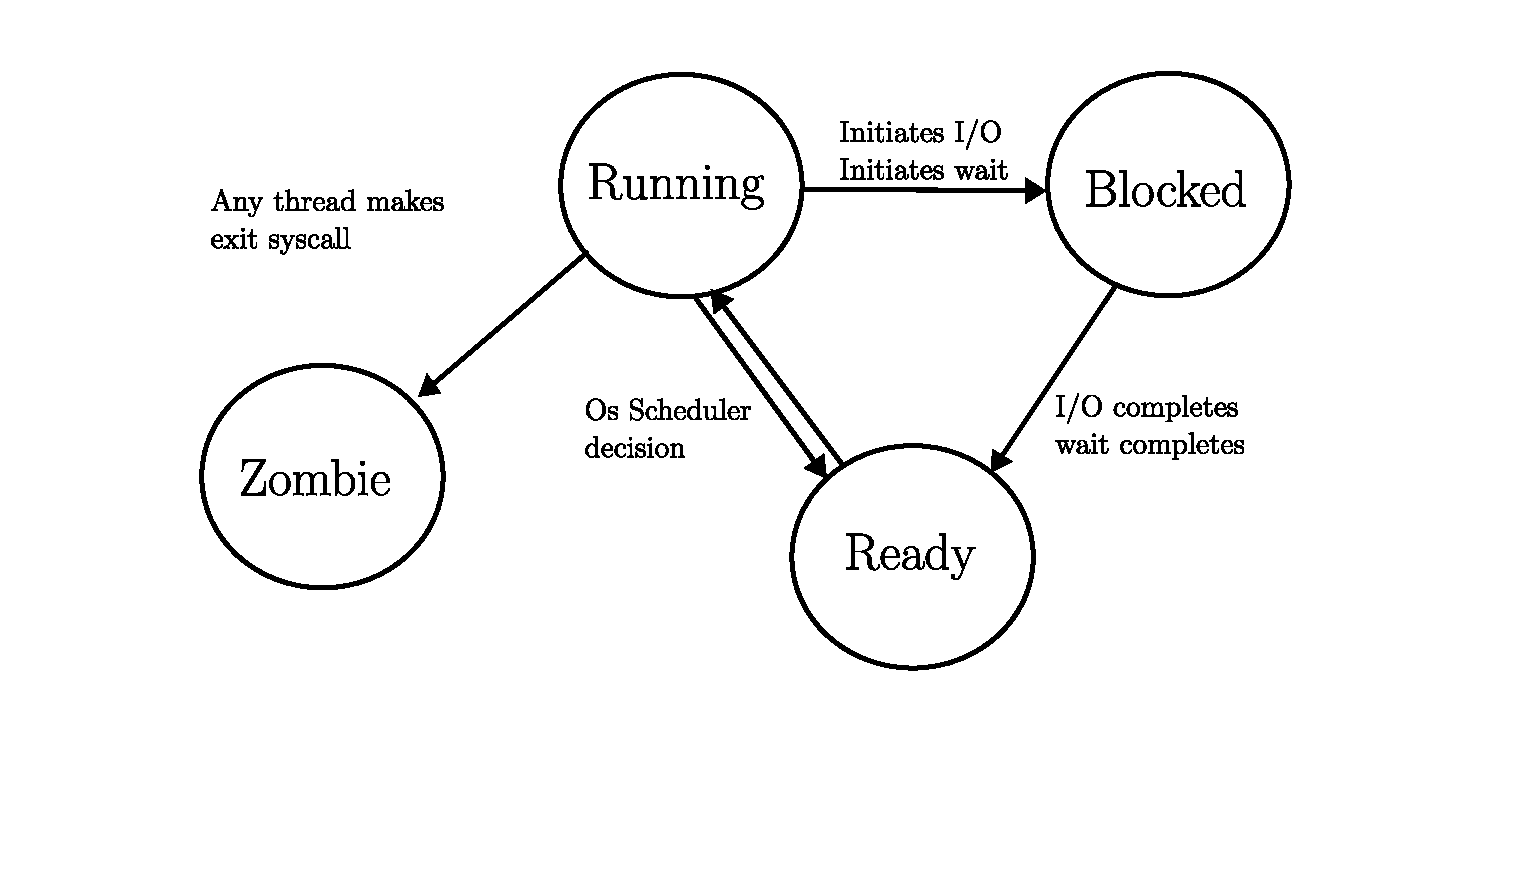
\includegraphics[width=0.9\textwidth]{figure/2026-05-06.pdf}
\caption{Process state diagram}
\end{figure}

\begin{parag}{Multiple forks}
    We can have multiple forks done at the same time, (one after another) using this we will create a tree of process. (as the child of the first work will call the next fork instruction itself etc...)
\end{parag}

\begin{parag}{File descriptor}
    As we have already seen that when forking, we are effectively copying all the thing image with the new thread. The question that comes up is what about the file descriptor, usually they are uniquely defined within a process. So when we will copy them, what will happen? In our case as a child process has an identical set of file descriptors, they will also be referring to the  \important{same resources}.
	
\end{parag}

\paragraph{Summary}%
\label{par:Summary}
\begin{parag}{CPU caching \& memory hierarchy}
    \begin{itemize}
        \item Reduces the amount of time that the CPU waits for memory access to complete
        \item Modern architecture typically have three caches: L1, L2 and L3
        \item Together with the main memory, they form the computer's memory hierarchy.
    \end{itemize}
\end{parag}

\begin{parag}{Memory virtualisation}
    Memory virtualisation works through address translation, implemented by the Memory Management Unit (MMU). We have three implementations possible 
	\begin{enumerate}
		\item Base \& Bound
		\item Segmentation
		\item Paging
	\end{enumerate}
	
	It allows the illusion that the process thinks it is occupying the main memory alone. And it is a \important{safe} illusions as each process can only touch its own memory image.
\end{parag}



\section{Virtualization}
The goal of this section is to see the Virtualization fundamentals (definition multiplexing, aggregation, emulation). We will also see an introduction to virtual machine.

\subsection{Virtualization Fundamentals}

\begin{center}
    \textit{Any problem in computer science can be solved by adding a level of indirection. But this usually creates another problem.}
\end{center}
Virtualization applies indirection to \important{layering} when the layred abstraction is \important{compatible} with the layer it relies upon.

\begin{framedremark}
I didn't get that sentence so I will debug it using some chatgpt text.\\
$ $\\
Key terms:
\begin{itemize}
    \item '\textit{indirection}' $= $inserting an extra intermediary layer
    \item '\textit{layering}' $ = $ building one abstraction on top of another
    \item '\textit{compatible}' $ =  $ the upper layer can behave as if the lower layer were the original expected system
\end{itemize}
The normal stack goes 
\begin{center}
    Application \textrightarrow OS \textrightarrow Hardware
\end{center}
With Virtualization
\begin{center}
    Application \textrightarrow Guest OS \textrightarrow Virtual Machine Monitor \textrightarrow Hardware
\end{center}
The hypervisor is the 'level of indirection'
\end{framedremark}



\begin{parag}{Layered \& Compatible}
	A virtualization layer exports the same (or a compatible) abstraction as the layer it relies on. It does so by hiding the physical names from the abstraction to ensure isolation.\\
	$ $\\
	Virtualization enforces modularity and can be applied to different types of resource (e.g., CPU, Memory...)
\end{parag}


\paragraph{3 main virtualization mechanisms}%
\label{par:3 main virtualization mechanisms}
There exists three different way to introduce virtualization into a system.
\begin{parag}{Multiplexing}
    We expose only a single ressource among multiple virtual entities (This is what is done with memory).
\end{parag}
\begin{parag}{Aggregation}
    We make multiple ressources appear as one single virtual resource (e.g., disk volumes)
\end{parag}
\begin{parag}{Emulation}
    We make a physical resource appear as another physical resources. This is what is being done with serial port over a USB port, or over SSH.
\end{parag}

\begin{parag}{What you can do with virtual memory}
	\begin{subparag}{Isolation \& context switching (process abstraction)}
       We can enforce modularity across address spaces (as seen in previous section). To do so the OS changes the page table base (priviledge instruction). Then we flush the MMU\\
   \end{subparag}
   \begin{subparag}{Demand paging}
       
	   Demand paging mean, that pages are loaded into RAM only when actually needed. Suppose a program accesses a virtual page that is not currently in RAM. Then 
	   \begin{enumerate}
	       \item MMU detects missing mapping
	       \item CPU raise a page fault
	       \item OS page fault handler runs
	       \item Os loads the page from disk
	       \item OS updates the PTE (Page Table Entry)
	   \end{enumerate}
	   When we say '\textit{change PTE and reload MMU}', what this mean in practice is that the OS updates the mapping so that the virtual page is up to date and can points to real physical page.
   \end{subparag}
   \begin{subparag}{Copy on Write}
       When a \texttt{fork()} creates a child process, copying all memory immediately would be expensive. Instead:
	   \begin{itemize}
	       \item Parent and child initially share the same physical pages
	       \item Both mapping are marked read-only
	   \end{itemize}
	   If one process writes:
	   \begin{enumerate}
	       \item Page fault occurs
	       \item OS allocates a new physical page
	       \item Os copies the old content
	       \item OS updates the writer's PTE
	       \item page becomes writable again
	   \end{enumerate}
	   This is what 'copy on write' means, the actual copy happens only when modification occurs.
	   
	   
	   
   \end{subparag}
\end{parag}



\subsection{Aggregation and Emulation}
\paragraph{Aggregation}%
\label{par:Aggregation}
The primary use of aggregation is to aggregate physical ressource together. Usually a computer has multiple memory module (DIMM). To be able to deal with those together, the memory controller aggregates the physical memory into a single namespace (typically contiguous).. (Here we are talking about the RAM, the stick that are plugged in the motherboard (if you are lucky to have more than one...)). But a computer also have many hard drives, we resolve that issue using RAID (Redundant Array of Inexpensive Disks) to make them appear as a single volume.
To see RAID implementation and volume

\paragraph{Emulation}%
\label{par:Emulation}
The goal of virtualization via \important{emulation} is to use software to emulate a resource different from the underlying ressource. We expose it within the OS as a virtual resource. Here are some example:
\begin{itemize}
    \item A \important{RAM disk}: P = DRAM, V = disk to mount a filesystem (/tmp)
    \item A \important{Java Virtual Machine}: P=x86-64 or Arm CPU; V=Java byte code
\end{itemize}


\subsection{Virtual Machines}
	\begin{center}
	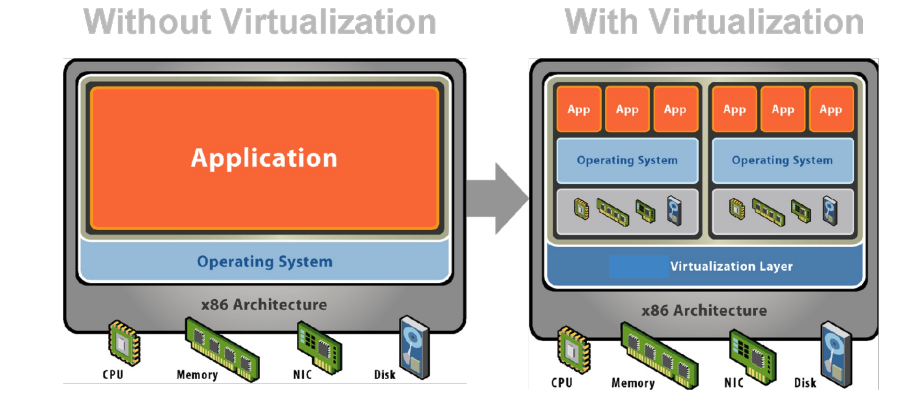
\includegraphics[scale=0.3]{screenshots/2026-05-13.png}
	\end{center}
	The idea is to apply virtualization principle to \important{an entire computer system}. But first some definition 
	\begin{definition}{Virtual machine}
	A virtual machine is an efficient, isolated duplicate of the real machine.
	\end{definition}
	There is always a virtual machine monitor (or hypervisor) which is always in complete control of the system, uses the hardware directly so that programs show at most a minor decrease in speed.
\begin{parag}{Terminology}
    \begin{subparag}{Operating system}
		\begin{itemize}
		    \item \important{Guest operating system}: running inside a virtual machine
		    \item \important{Host operating system}: running directly on the hardware combined with the VMM
		\end{itemize}
    \end{subparag}
	\begin{subparag}{Memory}
	    \begin{itemize}
	        \item Virtual memory ,as commonly understood
	        \item \important{Guest physical memory}: physical memory of the VM
	        \item \important{Host physical memory}: (actual) physical memory
	    \end{itemize}
	    
	\end{subparag}
\end{parag}

\begin{parag}{Type 1 vs Type 2}
    There is two possibilities when implementing VM. The first one is having the VMM also being the host OS (done on e.g., Xen, vSphere). Or the VMM is an optional extension to the host OS (e.g. KVM and Linux)
	\begin{center}2026-05-132026-052026-05-13
	\includegraphics[scale=0.3]{scr2026-05-13333-05-13_1.png}
	\end{center}
\end{parag}


\subsection{VMM Construction}
When building a VMM we will use both multiplexing and emulating. We will multiplex the CPU and Memory, (\important{with specific hardware support}) where 
\begin{itemize}
    \item Each VM has it own virtual CPUs (=virtual core), it requires system-level limited direct execution
    \item Each VM has its own guest physical memory (it relies on extended page tables)
\end{itemize}
And then we will emulate all the I/O devies (virtual disk, virtual keyboard, virtual screen, virtual ethrnet switch, etc.)\\
$ $\\
\begin{parag}{Limited direct execution}
    As seen previously, application can only executes unpriviledge execution, to be able to execute priviledge one, we use syscall which ask the kernel to do the jobs for us. But now this is different as we are adding a level of indirection. What we could do is to add a full layer
	\begin{center}
	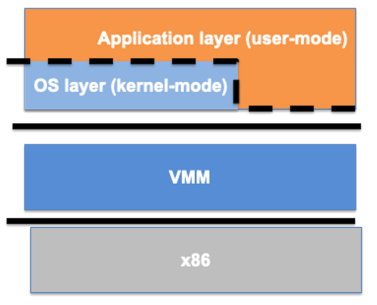
\includegraphics[scale=0.3]{screenshots/2026-05-13_2.png}
	\end{center}
	We will use the trick to expose the same abstraction $V$ as the underlying resource $P$ and therefore, everything else will still work as below. However this is not very fast right, everytime we have to go up and down the whole stack. A way to skip this is to allow the application layer and the guest OS to use the CPU directly (we will still trap some privileged instructions)
	\begin{center}
	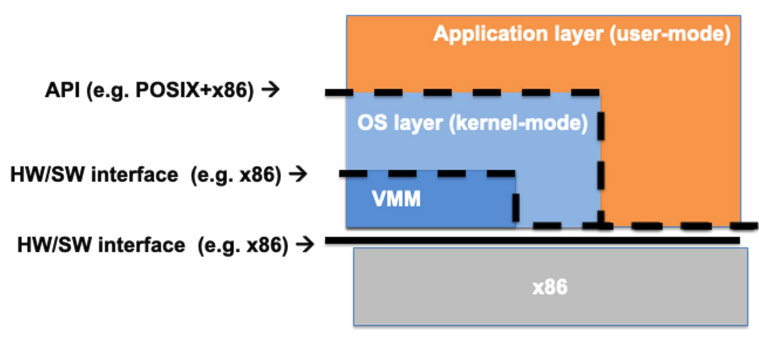
\includegraphics[scale=0.3]{screenshots/2026-05-13_3.png}
	\end{center}

\end{parag}

\begin{parag}{Virtual CPU --recap}
    Multiplexed in space and time --very much like kernel threads 
	\begin{itemize}
	    \item Space: VMM schedules vCPU from different VMs on different core
	    \item Time: VMM schedules multiple vCPUs on a limited set of physical cores 
	\end{itemize}
	Isolation is guaranteed via:
	\begin{itemize}
	    \item Non-root mode execution of the VM
	    \item Host OS/VMM is presumed to be correct (very much like the OS)
	\end{itemize}
	
	
\end{parag}



\begin{parag}{Virtualizing physical memory}
    \begin{center}
    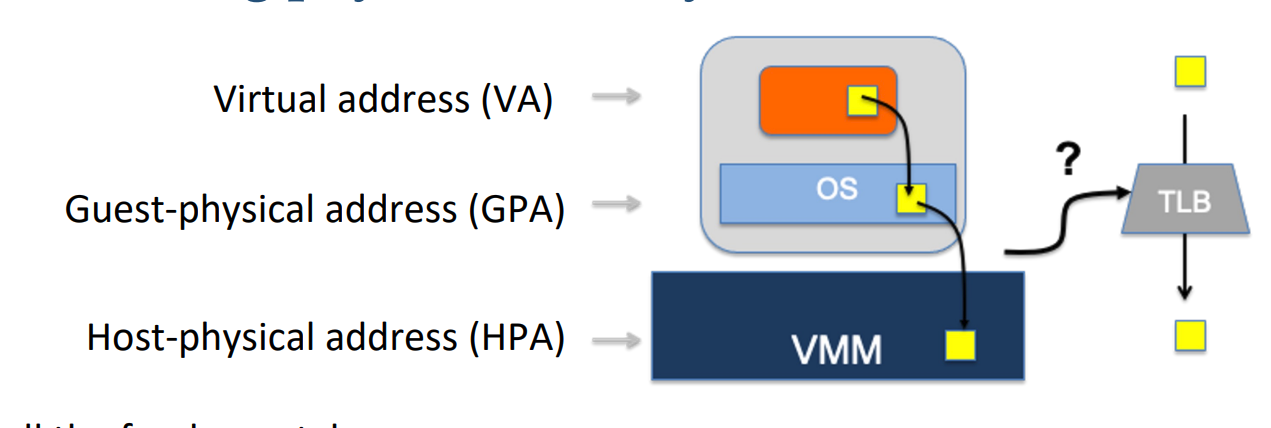
\includegraphics[scale=0.3]{screenshots/2026-05-13_4.png}
    \end{center}
	Recall the fundamentals 
	\begin{itemize}
	    \item Processor use VA
	    \item TLB stores mapping between VA and HPA
	    \item Architecture determins how TLB is loaded (e.g., page table walk)
	\end{itemize}
	
\end{parag}

\begin{parag}{Extended (or nested) page tables}
    Hardware simultaneously walks through two page table structures
	\begin{itemize}
	    
	    \item One tree, controlled by the guest, containing GPA
	    \item One tree, controlled by the VMM, continuing HPA
	    \item Simultaneous walk requires \important{quadratic number of references}
	    \item Implemented in hardware, with dedicated caches to improve performance
	\end{itemize}
	

\end{parag}



\begin{parag}{Summary}
    There is two independent page table trees
	\begin{itemize}
	    \item It allows for independent management by the isolated entities (guest OS and VMM)
	    \item Architecture implies a quadratic number of references
	\end{itemize}
	It also gives us a minor performance overhead 
	\begin{itemize}
	    \item TLB hit - no performance penalty
	    \item TLB miss -- minimize actual number of memory references through
	\end{itemize}
	
	
\end{parag}











\end{document}


